%\part*{Lezione 15/02/2021}
\chapter{Nozioni principali}
In questo capitolo introduciamo i concetti principali della fisica nucleare a grandi linee. Questo capitolo copre la lezione del 15/02/2021.
\section{Binding Energy}
\subsection{Notazione} 
Dato un nucleo $X$ con $Z$ protoni, $N$ neutroni e $A=Z+N$ numero di massa, si utilizza la notazione\footnote{Da notare che la notazione è ridondante: sarebbe infatti sufficiente dare $A$ e $X$ o $A$ e $Z$ o $N$ e $Z$,\dots}:
$$\ce{^{A}_{Z}X_N}$$

\begin{definition}[\textbf{Energia di Legame}]
Si definisce \textbf{energia di legame} o \textbf{binding energy}\index{binding energy}\footnote{Si pone $c=1$.}:
$$B(Z,A) = Z m_p + N m_N - m \,(\ce{^{A}_{Z}X_N})>0\qquad \text{è definita positiva}$$
\end{definition}
\noindent Misurando la massa del nucleo $m (\ce{^{A}_{Z}X_N})$, possiamo studiare l'andamento di $B/A$ in funzione di $A$ e ottenere una curva come quella in Figura \ref{B/A}.

\begin{figure}[h]
    \centering
    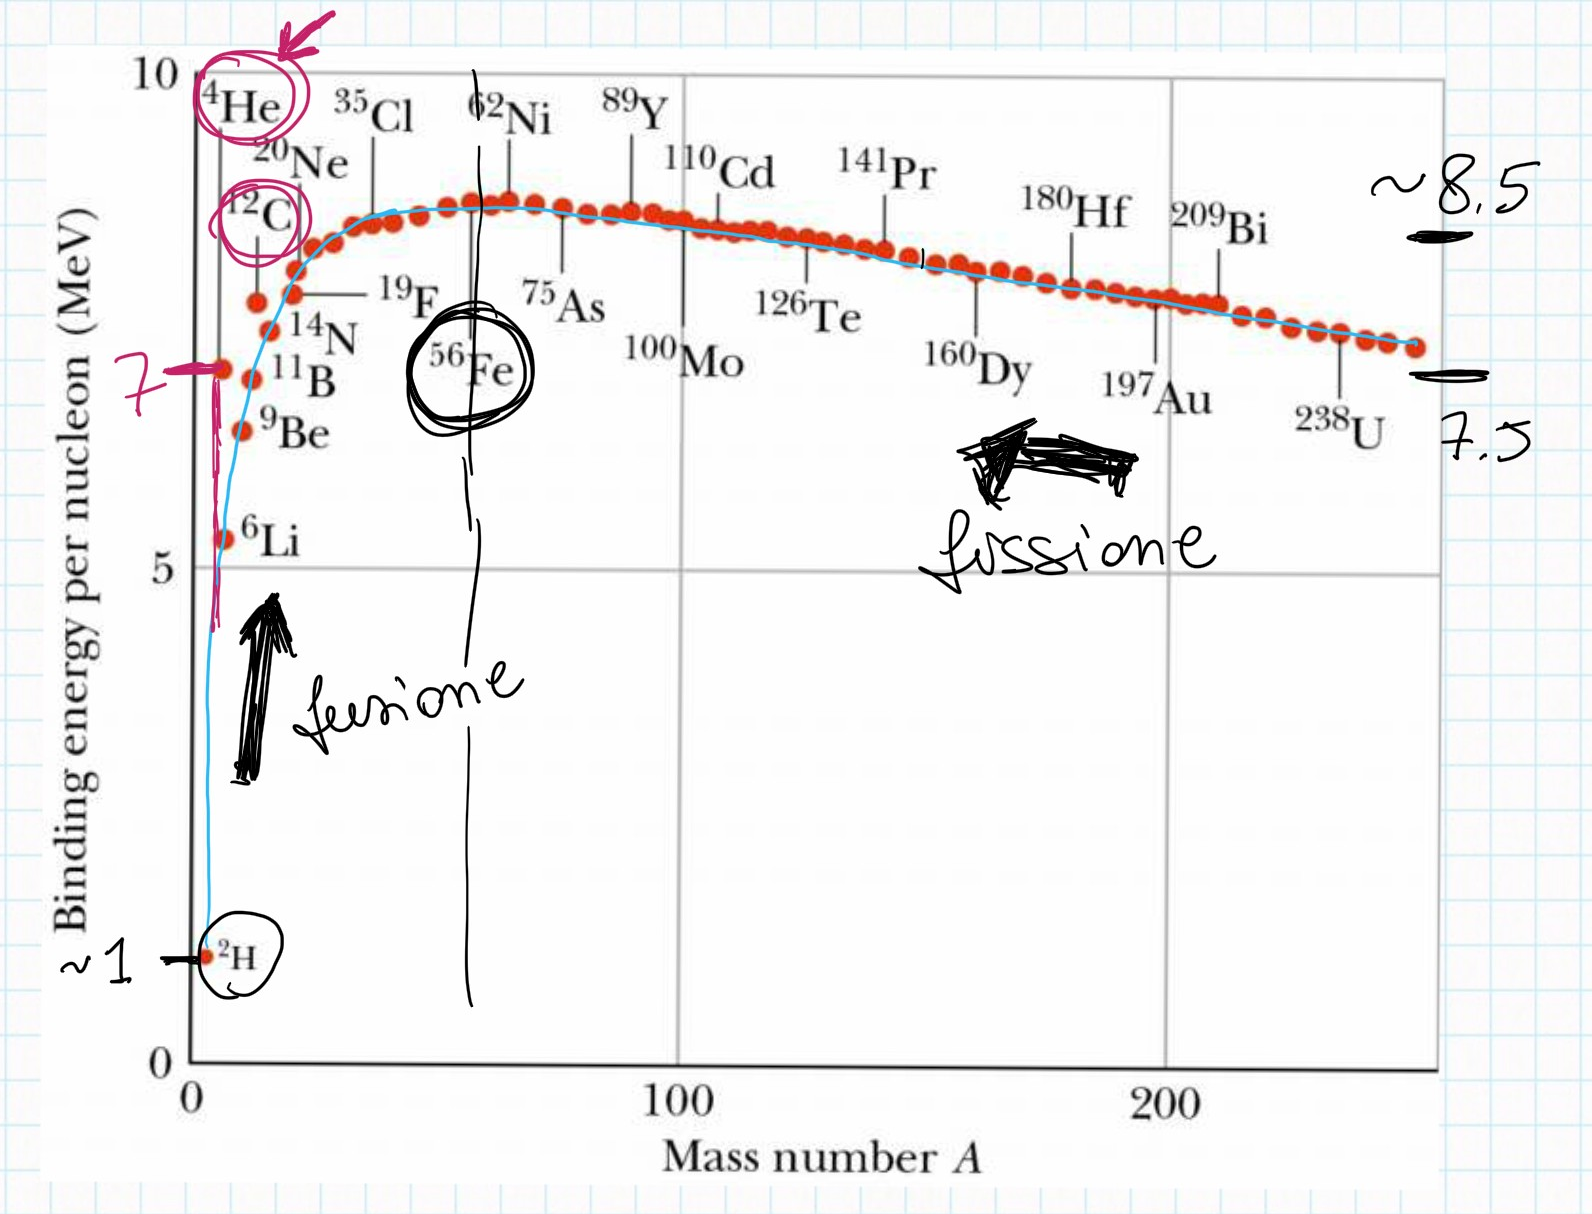
\includegraphics[scale=0.26]{Immagini/curva_elementi.png}
    \caption{Curva che rappresenta l'andamento dell'energia di legame (per nucleone) al crescere del numero di massa. Sono segnati il picco del ferro, le reazioni in funzione dei pesi atomici e i salti dei nuclei di elio e carbonio.}
    \label{B/A}
\end{figure}

\subsection{Primi passi} 
Il primo stato legato possibile è lo stato $pn$ ($A=2$), ovvero $\ce{^2_1H_1}$, che ha una $B\simeq 2.2245$ MeV\footnote{Altri parametri caratteristici del deutone\index{deutone}:%
\begin{align*}%
    &J^\pi = 1^+ & S=1,\, &T= 0,\, \ell = 0,2 \\
    &r_d \simeq 1.975 \unit{fm} & &A_S \simeq 0.8781 \unit{fm}^{-1/2} \\
    &\mu_d \simeq 0.8574\;\mu_N & &Q_d \simeq 0.2859 \unit{fm}^2 
\end{align*}%
dove abbiamo chiamato il magnetone nucleare\index{magnetone nucleare@magnetone nucleare $\mu_N$} $\mu_N = e^2\hbar/2m_p c$.}%
; notiamo poi un picco nei d'intorni del $\ce{^56Fe}$:
\begin{itemize}
    \item Per $A<56$ allora si ha che \vir{salendo} anche l'energia di legame aumenta, dunque è favorita la \textbf{fusione nucleare}\footnote{Fa eccezione l'elio per cui si ha una $B\sim 28$ MeV; cercheremo di spiegare più avanti il motivo. Lo stesso vale per il carbonio.}:
    $$\ce{^{A_1}X} + \ce{^{A_2}Y} \to \ce{^AX}'$$
    \item Per $A>56$ \vir{salire} non è conveniente e vengono quindi privilegiati i processi di \textbf{fissione nucleare}:
    $$\ce{^AX}' \to \ce{^{A_1}X} + \ce{^{A_2}Y}$$
\end{itemize}
\noindent Osserviamo anche che eccetto i primi salti la curva si assesta intorno a valori compresi tra i $7.5 \div 8.5$ MeV per cui consideriamo per la maggior parte degli elementi il valor medio di 8 MeV.

\section{Formula Semi-empirica di massa}
Per $A$ \vir{sufficientemente grande} esiste una formula empirica che \textit{fitta} abbastanza bene i dati.
\begin{definition}[\textbf{Formula Semi-empirica di Massa}]\index{formula semi-empirica di massa}
Esprime l'energia di legame per nuclei pesanti:
$$B = \underbrace{a_V \, A - a_S\, A^{2/3} - a_C \, \frac{Z(Z-1)}{A^{1/3}}}_\text{Modello a goccia} %
- \underbrace{a_{sym} \, \frac{(A-2Z)^2}{A}}_\text{Modello a shell nucleare} %
+\, \delta$$
\begin{displaymath}
\begin{aligned}
&\text{\textbf{Termine di Volume}} & &a_V = 15.5\;\mbox{MeV} & &\text{\textbf{Termine di Coulomb}} & &a_C = 0.72\;\mbox{MeV}\\
&\text{\textbf{Termine di Superficie}} & &a_S = 16.8\;\mbox{MeV} & &\text{\textbf{Termine Simmetrico}} & &a_{sym} = 23\;\mbox{MeV}\\
\end{aligned}
\end{displaymath}
\begin{displaymath}
\begin{aligned}
&\text{\textbf{Termine di Pairing}} & &\delta = \Biggl \{ 
\begin{array}{ll}
    34\;\mbox{MeV}\;\, A^{-3/4} &  \text{even-even}\\
    0 &  A\; \text{dispari}\\
    -34\;\mbox{MeV}\;\, A^{-3/4} & \text{odd-odd}
\end{array}
\end{aligned}
\end{displaymath}
\end{definition}
Passiamo adesso a illustrare il significato dei singoli coefficienti:
\begin{itemize}
    \item $a_V$:\index{formula semi-empirica di massa!termine di volume} il primo termine è lineare in $A$, dal momento che l'interazione nucleare è a corto raggio, ovvero è un'interazione di primi vicini. Si chiama termine di volume, infatti il raggio nucleare scala\footnote{$r_0\sim 1.2$ fm.} come $r\simeq r_0 A^{1/3}$, di conseguenza il volume scala con $A$.
    \item $a_S$:\index{formula semi-empirica di massa!termine di superficie} i nucleoni sulla \vir{superficie} hanno ovviamente meno vicini di quelli più \vir{interni}, dunque dobbiamo tenere conto di questa assenza con un termine proporzionale alla superficie, cioè, dall'andamento visto prima, proporzionale a $A^{2/3}$.
    \item $a_C$:\index{formula semi-empirica di massa!termine di Coulomb} poiché la formula vale per atomi pesanti, spesso $Z\gg 1$ e il termine coulombiano viene riscritto come:
    $$a_C \frac{Z^2}{A^{1/3}}$$
    Questo deriva dall'espressione dell'energia coulombiana $\sim q^2/R = Z^2 e^2 / (r_0A^{1/3})$; allora $a_C \propto e^2/r_0$.
    \item $a_{sym}$:\index{formula semi-empirica di massa!termine simmetrico} questo è un termine puramente quantistico e può essere riscritto come\footnote{Si usa solo $A=Z+N$.}:
    $$(A-2Z)^2 = (N-Z)^2$$
    Si vede allora che per $N=Z$ questo termine non contribuisce, ovvero il nucleo è più stabile; ciò è confermato dalle osservazioni solo per $A$ \vir{non troppo grandi}, come si vede in Figura \ref{segre}, quindi per tenerne conto si divide per $A$.
    \item $\delta$: esistono solo 6 nuclei stabili in natura con $A$ pari e $N$ e $Z$ dispari.
\end{itemize}
\noindent Infine valgono le seguenti disuguaglianze:
$$a_C \lll a_V <a_S < a_{sym}$$

\begin{figure}[h]
    \centering
    \textbf{\Large Carta di Segré}\index{carta di Segré}\par\medskip
    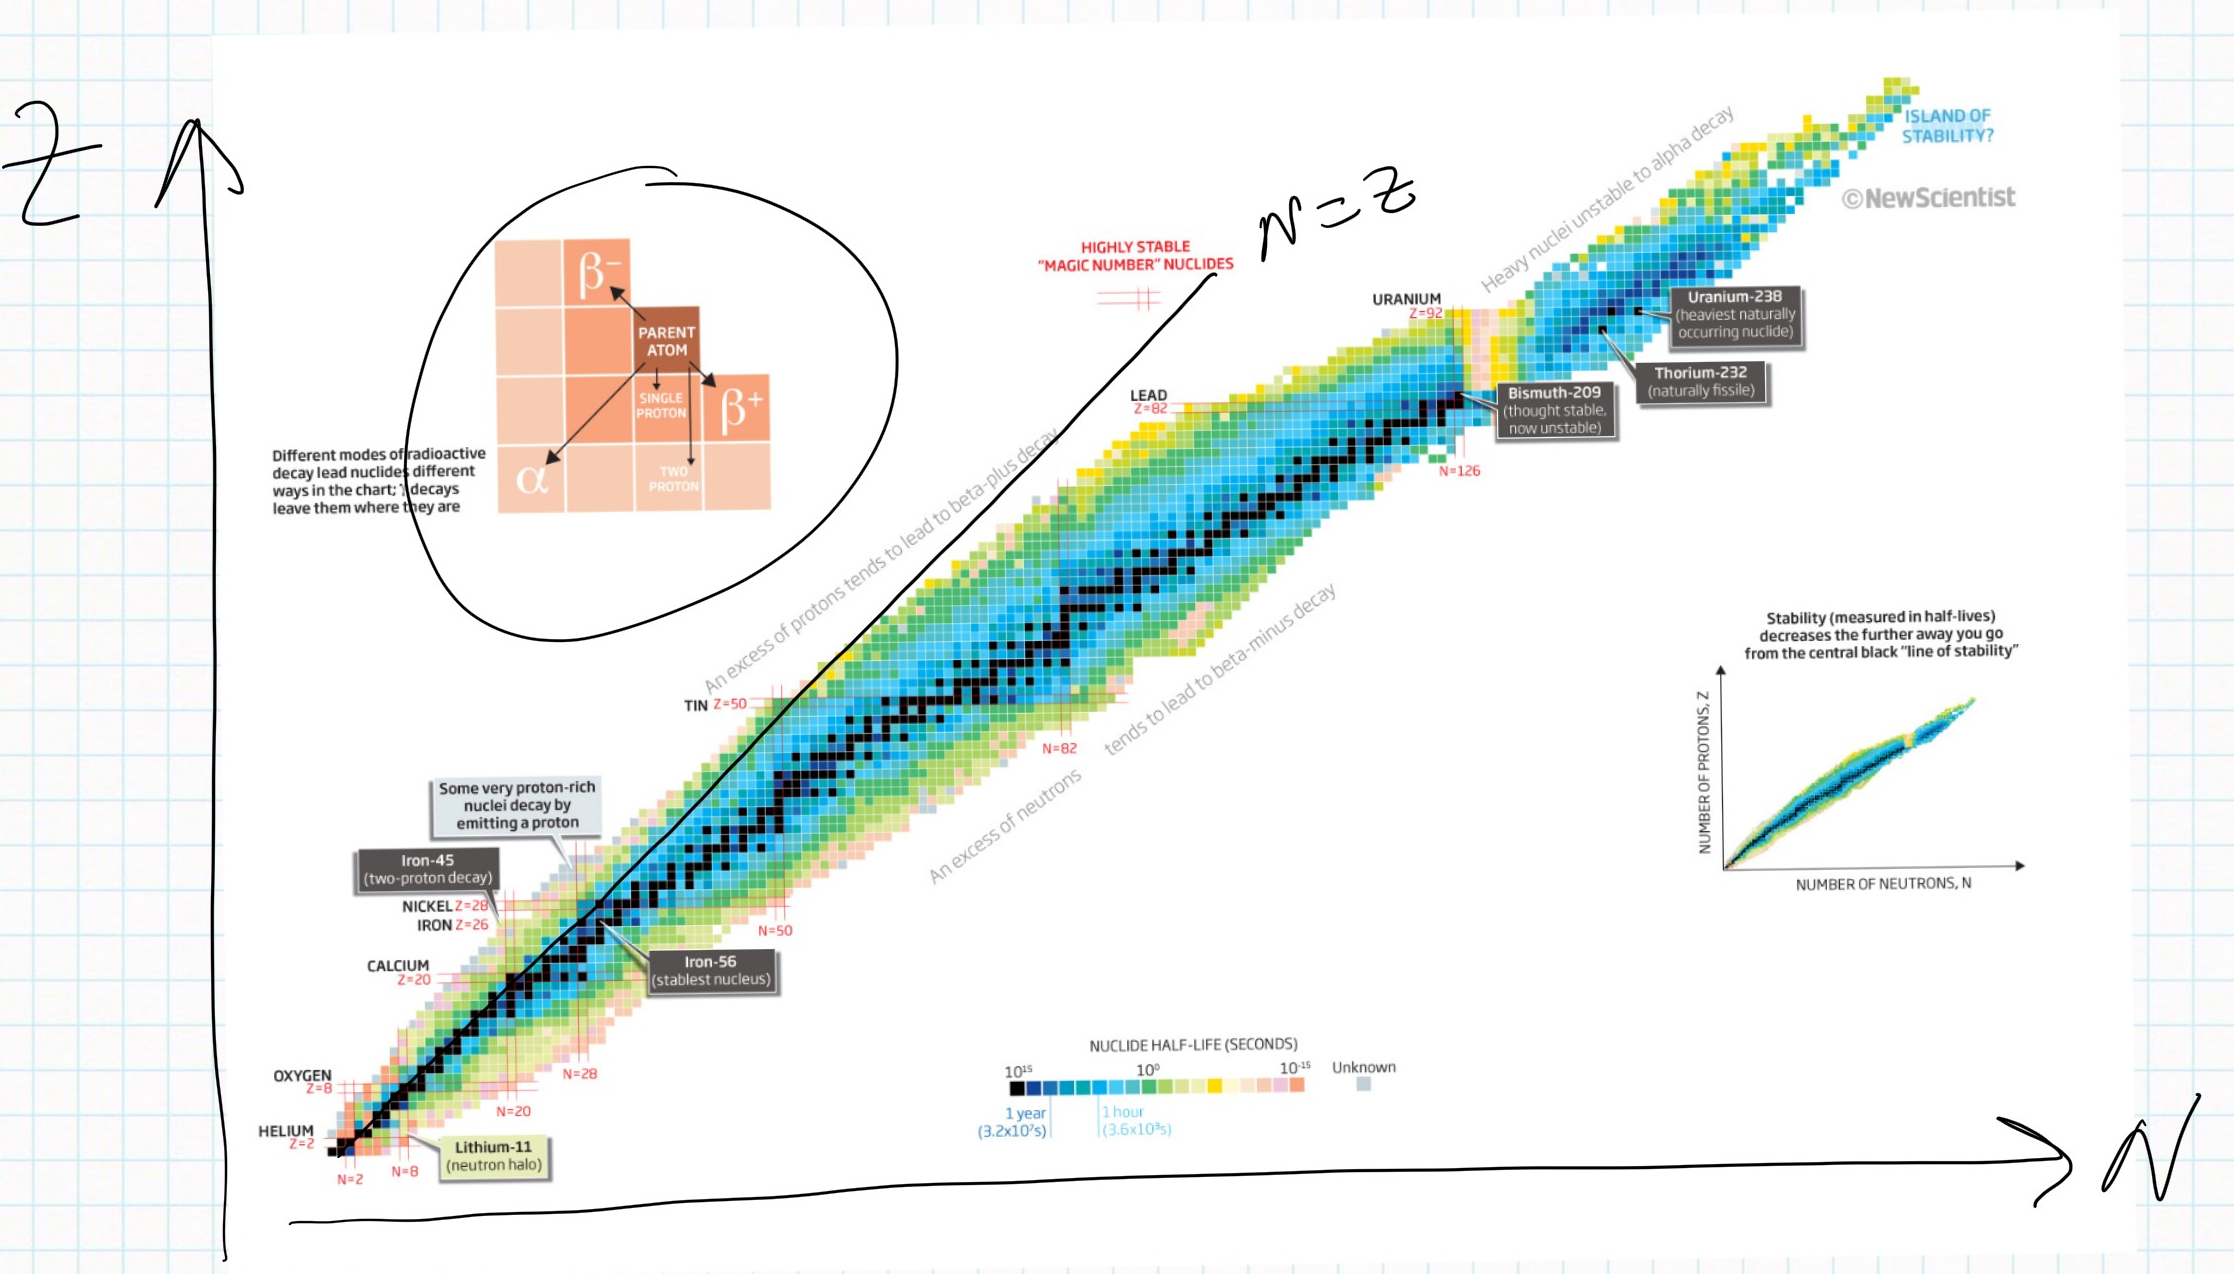
\includegraphics[scale=0.21]{Immagini/Segre.png}
    \caption{Sono riportati i nuclei in base a $Z$ e $N$. La linea centrale viene chiamata \textbf{valle di stabilità}\index{valle di stabilità}. Indicativamente dopo il Ca non vale più $N=Z$ per i nuclei stabili, ma $N>Z$. In alto sono riportati i decadimenti.}
    \label{segre}
\end{figure}

\newpage

\section{Panoramica sui decadimenti}
Illustriamo i principali decadimenti\footnote{Il decadimento $\gamma$ non è riportato, tuttavia approfondiremo i vari decadimenti nel Capitolo \secrif{sec-decadimenti}.}.

\paragraph{Decadimento $\alpha$} Mediato dall'interazione forte (stato iniziale e stato finale presentano solo nuclei), è descritto da:
$$\alpha: \qquad \ce{^A_ZX_N} \to \ce{^{A-4}_{Z-2}Y_{N-2}} + \alpha $$
Non lo tratteremo.
\paragraph{Decadimenti $\beta$} Mediati dall'interazione debole (presenza del neutrino):
$$\beta^-: \qquad \ce{^A_ZX_N} \to \ce{^{A}_{Z+1}Y_{N-1}} + e^- + \bar{\nu}_e \quad \text{Dentro il nucleo}\quad n \to p + e^- + \bar{\nu}_e $$
$$\beta^+: \qquad \ce{^A_ZX_N} \to \ce{^{A}_{Z-1}Y_{N+1}} + e^+ + \nu_e \quad \text{Dentro il nucleo}\quad p \to n + e^+ + \nu_e$$

\section{Una parentesi: la stabilità}
Procediamo adesso con una \vir{dimostrazione} della stabilità dei nuclei con $N=Z=A/2$ per $Z\lsim 20$.\\
Per primo scriviamo la massa di un generico nucleo in funzione di $Z$ e $A$:
$$m(\nuc{X}{A}{Z}{N}) = Zm_p + Nm_n - B(Z,A) \simeq Z m(\ce{^1H}) + (A-Z)m_n- B(Z,A)$$
Fissato $A$ cerchiamo il minimo di $m$ al variare di $Z$.
$$\frac{\partial m}{\partial Z} = 0 \;\Rightarrow\; m(\ce{^1H})-m_n + 2a_C \frac{Z}{A^{1/3}} - \frac{a_C}{A^{1/3}}-4a_{sym}\frac{A-2Z}{A} = 0$$
$$Z_{\min} = \frac{m_n - m(\ce{^1H})+a_C A^{1/3}+4 a_{sym}}{2[a_CA^{1/3}+4a_{sym}A^{-1}]}\simeq \frac{A}{2}$$
dove nell'ultima approssimazione abbiamo usato che $m(\ce{^1H})\simeq m_n$ e che $a_C\ll a_{sym}$, per cui per $A$ piccolo (ma non troppo) si può trascurare il termine $a_C A^{1/3}$ nel denominatore.\\
Dato che l'andamento di $B\propto Z^2$ allora possiamo rappresentare\footnote{Qui trattiamo $Z$ come una variabile continua per ottenere gli andamenti.} approssimativamente l'andamento di $m$ al variare di $Z$ come in Figura \ref{MvsZ}\footnote{È molto raro ma è possibile osservare anche un decadimento doppio $\beta$ indicato $2\nu\beta\beta$; quello che si cerca di osservare è un doppio $\beta$ senza neutrino, ovvero $\phi \nu \beta\beta$, poiché in questo caso si avrebbe una violazione dello \textit{standard model}, il neutrino non sarebbe una particella di Dirac, ma di Mayorana per cui $\nu = \bar{\nu}$.}.

\begin{figure}[!h]
    \centering
    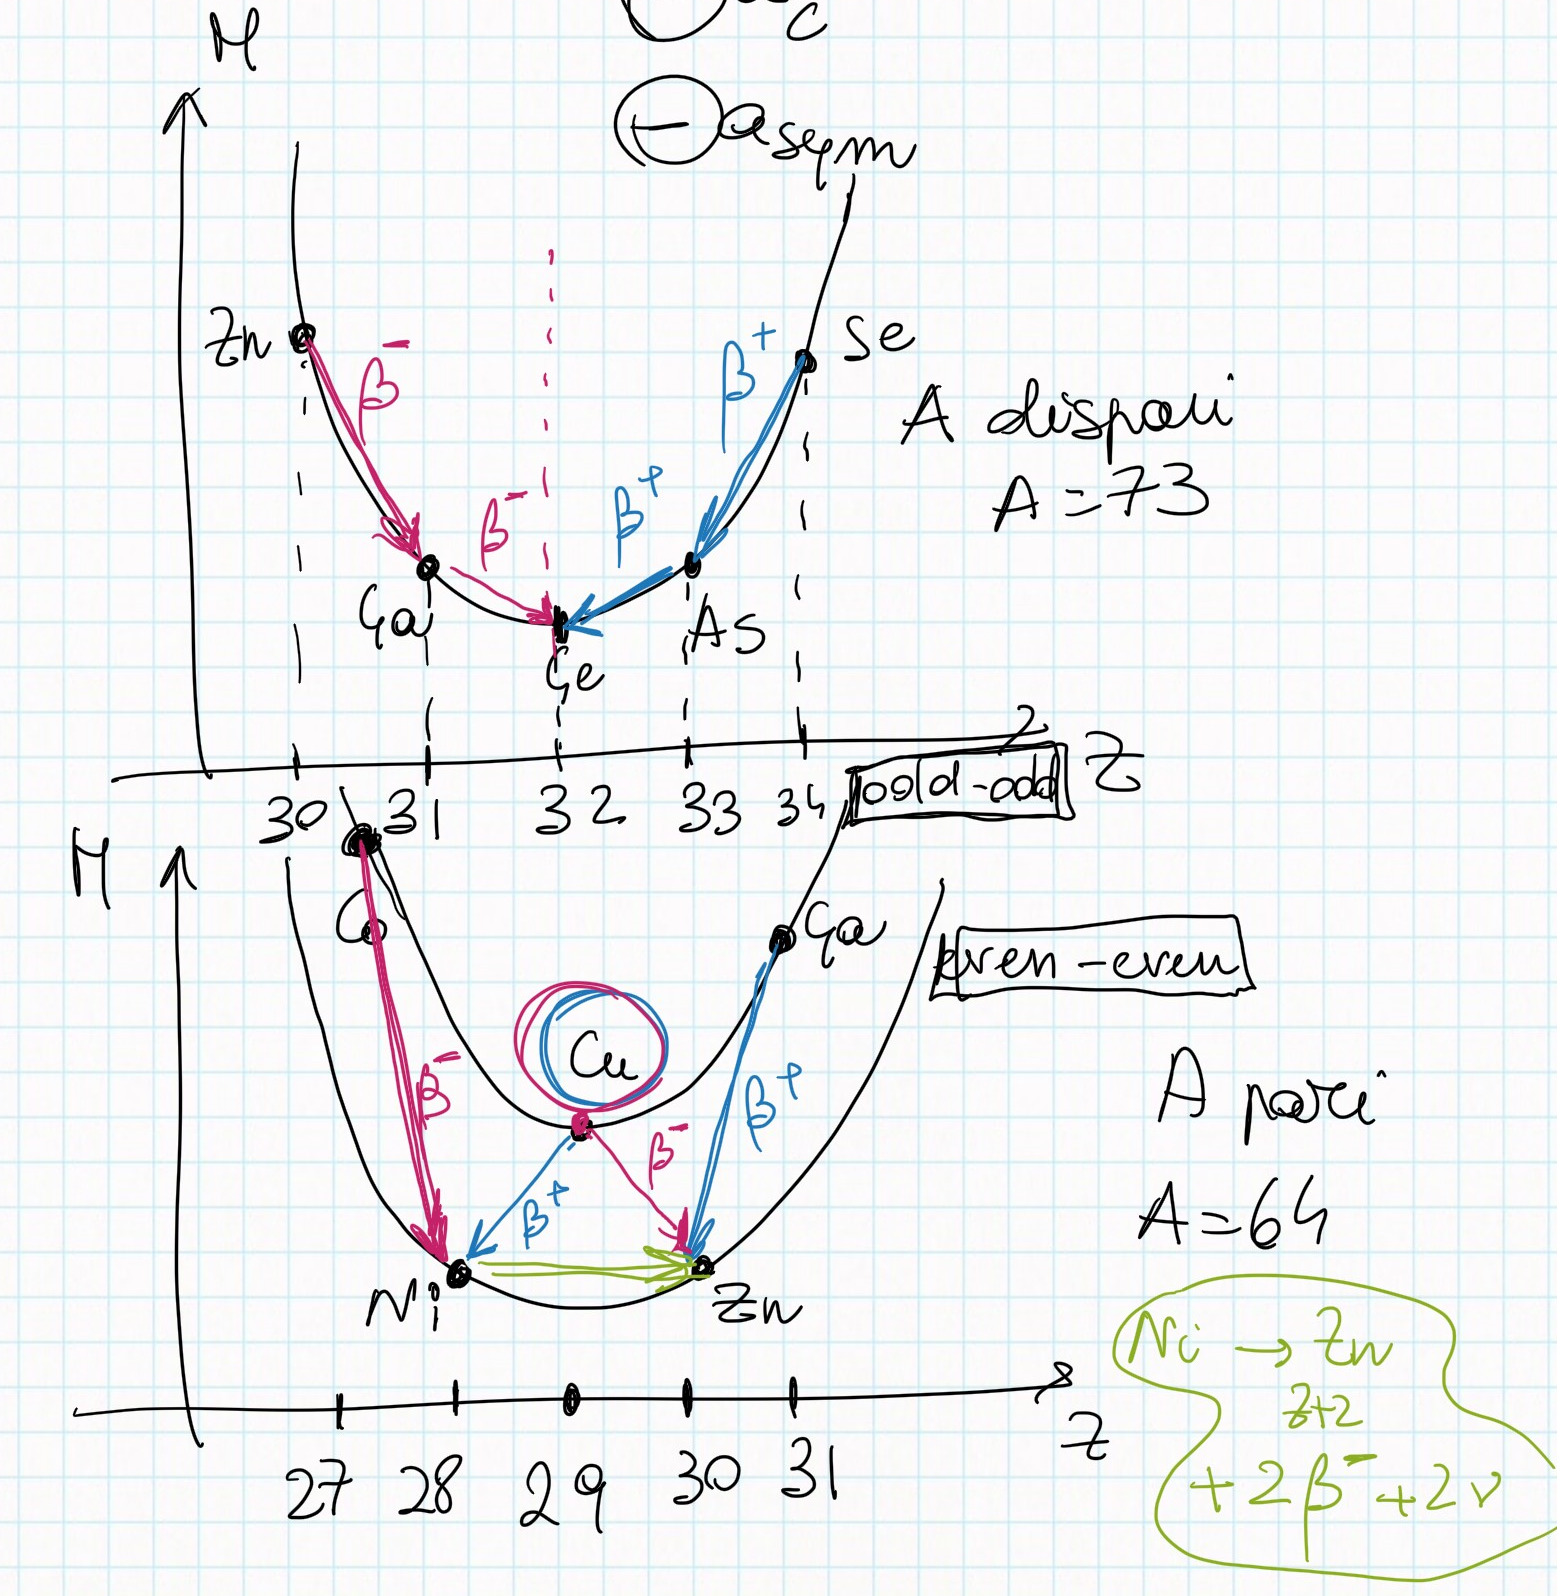
\includegraphics[scale=0.3]{Immagini/MvsZ.png}
    \caption{Rappresentazione di $m\equiv M$ in funzione di $Z$. Si osserva che per i nuclei con $A$ dispari si hanno decadimenti $\beta^-$ scendendo verso destra, mentre $\beta^+$ scendendo verso sinistra. Per i nuclei con $A$ pari il termine di pairing nell'energia di legame si fa sentire e questo porta a nuclei che possono avere sia $\beta^+$ che $\beta^-$ (in questa configurazione i doppio $\beta$ sono talmente \vir{poco probabili} da poter essere trascurati).}
    \label{MvsZ}
\end{figure}

\begin{curiosita}
In Fisica Medica viene utilizzato il $\ce{^64Cu}$ poiché può sia decadere $\beta^+$ che $\beta^-$; il decadimento $\beta^+$ viene usato per la PET, mentre il $\beta^-$ per la cura dei tumori.
\end{curiosita}

\section{$Q$-value}
Dato un processo\footnote{Come sempre $c=1$} $A+B\to C+D$ si definisce $Q$-value:
$$Q = m_A + m_B - m_C - m_D$$
Si hanno allora:
\begin{itemize}
    \item[-] $Q>0$ \textbf{esotermico} (spontaneo); l'energia relativa può essere nulla. 
    \item[-] $Q<0$ \textbf{endotermico} (non spontaneo); l'energia relativa dev'essere positiva.
\end{itemize}
\newpage

